\documentclass[11pt]{article}
\usepackage[margin=1in]{geometry}
\usepackage{graphicx}
\usepackage{booktabs}
\usepackage{float}
\usepackage{amsmath}
\usepackage{hyperref}
\title{COS 568 Assignment 2: Distributed Training of Language Models}
\author{NetID: od2961 \quad Liv d'Aliberti}
\date{March 20, 2026}

\begin{document}
\maketitle

\section{Setup and Reproducibility}
\begin{itemize}
\item Task 1 CPU run: 1 node (node701), backend \texttt{gloo}-free single-process training.
\item Task 1 GPU run: 1 node (node915), single GPU.
\item CPU distributed timing runs: Tasks 2(a), 2(b), and 3 on \texttt{node702, node703, node704, node705}; 1 rank per node, backend \texttt{gloo}.
\item CPU Task 4 profiling runs: \texttt{node706, node707, node708, node710}; 1 rank per node, backend \texttt{gloo}.
\item Multi-node GPU distributed runs: 4 nodes, 4 ranks, 1 rank per node, backend \texttt{nccl}.
\item GPU distributed nodes: \texttt{node105, node915, node916, node917}
\item Seed: \texttt{42}, PyTorch version: \texttt{2.9.1+cu128}, commit: \texttt{4444ce4}.
\end{itemize}

\section{Task 1: Single-Node Fine-Tuning}
\begin{table}[H]
\centering
\begin{tabular}{ccc}
\toprule
Epoch & CPU acc & GPU acc \\
\midrule
1 & 0.5920577617 & 0.5740072202 \\
2 & 0.6462093863 & 0.6389891697 \\
3 & 0.6534296029 & 0.6606498195 \\
\bottomrule
\end{tabular}
\caption{Task 1 evaluation accuracy after each epoch.}
\end{table}

\begin{table}[H]
\centering
\begin{tabular}{ccc}
\toprule
Minibatch & CPU loss & GPU loss \\
\midrule
1 & 0.748251 & 0.778352 \\
2 & 0.797213 & 0.785116 \\
3 & 0.708992 & 0.688311 \\
4 & 0.755476 & 0.738948 \\
5 & 0.740575 & 0.708527 \\
\bottomrule
\end{tabular}
\caption{Task 1 first five minibatch losses.}
\end{table}

\section{Tasks 2(a), 2(b), and 3}
\begin{table}[H]
\centering
\begin{tabular}{lcccc}
\toprule
Hardware & Task & Method & Avg iter time (s) & Timed iters \\
\midrule
CPU & 2(a) & gather+scatter & 27.086402 & 38 \\
CPU & 2(b) & all\_reduce & 11.063006 & 38 \\
CPU & 3 & DDP & 8.161475 & 38 \\
GPU & 2(a) & gather+scatter & 2.360095 & 38 \\
GPU & 2(b) & all\_reduce & 0.754817 & 38 \\
GPU & 3 & DDP & 0.603755 & 38 \\
\bottomrule
\end{tabular}
\caption{Average iteration time after dropping the first iteration.}
\end{table}

CPU Task 2(a) vs 2(b) max per-step loss difference: 1.788e-07.\\
GPU Task 2(a) vs 2(b) max per-step loss difference: 1.788e-07.

\begin{figure}[H]
\centering
\begin{minipage}[t]{0.48\linewidth}
\centering
\textbf{CPU Task 2(a)}\\[0.3em]
\includegraphics[width=\linewidth]{../outputs/report_runs_cpu_nodes/task2a/figures/loss_curve_all_ranks.png}
\end{minipage}\hfill
\begin{minipage}[t]{0.48\linewidth}
\centering
\textbf{GPU Task 2(a)}\\[0.3em]
\includegraphics[width=\linewidth]{../outputs/report_runs_gpu_nodes/task2a/figures/loss_curve_all_ranks.png}
\end{minipage}
\caption{Task 2(a) loss curves across all ranks.}
\end{figure}

\begin{figure}[H]
\centering
\begin{minipage}[t]{0.48\linewidth}
\centering
\textbf{CPU Task 2(b)}\\[0.3em]
\includegraphics[width=\linewidth]{../outputs/report_runs_cpu_nodes/task2b/figures/loss_curve_all_ranks.png}
\end{minipage}\hfill
\begin{minipage}[t]{0.48\linewidth}
\centering
\textbf{GPU Task 2(b)}\\[0.3em]
\includegraphics[width=\linewidth]{../outputs/report_runs_gpu_nodes/task2b/figures/loss_curve_all_ranks.png}
\end{minipage}
\caption{Task 2(b) loss curves across all ranks.}
\end{figure}

\begin{figure}[H]
\centering
\begin{minipage}[t]{0.48\linewidth}
\centering
\textbf{CPU Task 3}\\[0.3em]
\includegraphics[width=\linewidth]{../outputs/report_runs_cpu_nodes/task3/figures/loss_curve_all_ranks.png}
\end{minipage}\hfill
\begin{minipage}[t]{0.48\linewidth}
\centering
\textbf{GPU Task 3}\\[0.3em]
\includegraphics[width=\linewidth]{../outputs/report_runs_gpu_nodes/task3/figures/loss_curve_all_ranks.png}
\end{minipage}
\caption{Task 3 loss curves across all ranks.}
\end{figure}

\section{Task 4: Profiling and Communication Overhead}
\begin{table}[H]
\centering
\begin{tabular}{lcccc}
\toprule
Hardware & Method & Step & Total ms & Comm ms / pct \\
\midrule
CPU & gather\_scatter & 1 & 28165.536 & 21336.960 / 75.756\% \\
CPU & gather\_scatter & 2 & 27395.801 & 21310.518 / 77.788\% \\
CPU & gather\_scatter & 3 & 27446.430 & 21308.354 / 77.636\% \\
CPU & all\_reduce & 1 & 11357.282 & 5836.017 / 51.386\% \\
CPU & all\_reduce & 2 & 11057.445 & 5561.979 / 50.301\% \\
CPU & all\_reduce & 3 & 11137.599 & 5557.221 / 49.896\% \\
CPU & ddp & 1 & 8428.010 & 5639.442 / 66.913\% \\
CPU & ddp & 2 & 8175.506 & 5449.669 / 66.658\% \\
CPU & ddp & 3 & 8160.515 & 5271.923 / 64.603\% \\
GPU & gather\_scatter & 1 & 2445.820 & 2139.141 / 87.461\% \\
GPU & gather\_scatter & 2 & 2322.969 & 2177.100 / 93.721\% \\
GPU & gather\_scatter & 3 & 2321.385 & 2177.635 / 93.808\% \\
GPU & all\_reduce & 1 & 731.361 & 598.331 / 81.811\% \\
GPU & all\_reduce & 2 & 752.318 & 623.953 / 82.937\% \\
GPU & all\_reduce & 3 & 754.412 & 625.856 / 82.959\% \\
GPU & ddp & 1 & 621.920 & 546.223 / 87.828\% \\
GPU & ddp & 2 & 608.071 & 532.362 / 87.549\% \\
GPU & ddp & 3 & 605.935 & 531.832 / 87.771\% \\
\bottomrule
\end{tabular}
\caption{Per-step communication overhead from the profiled three-step windows.}
\end{table}

\begin{figure}[H]
\centering
\begin{minipage}[t]{0.48\linewidth}
\centering
\textbf{CPU gather scatter}\\[0.3em]
\includegraphics[width=\linewidth]{../outputs/task4_cpu_nodes/gather_scatter/figures/rank0_steps1to3_overview.png}
\end{minipage}\hfill
\begin{minipage}[t]{0.48\linewidth}
\centering
\textbf{GPU gather scatter}\\[0.3em]
\includegraphics[width=\linewidth]{../outputs/task4_gpu_nodes/gather_scatter/figures/rank0_steps1to3_overview.png}
\end{minipage}
\caption{Profiler overview for gather scatter over profiled steps 1-3.}
\end{figure}

\begin{figure}[H]
\centering
\begin{minipage}[t]{0.48\linewidth}
\centering
\textbf{CPU all reduce}\\[0.3em]
\includegraphics[width=\linewidth]{../outputs/task4_cpu_nodes/all_reduce/figures/rank0_steps1to3_overview.png}
\end{minipage}\hfill
\begin{minipage}[t]{0.48\linewidth}
\centering
\textbf{GPU all reduce}\\[0.3em]
\includegraphics[width=\linewidth]{../outputs/task4_gpu_nodes/all_reduce/figures/rank0_steps1to3_overview.png}
\end{minipage}
\caption{Profiler overview for all reduce over profiled steps 1-3.}
\end{figure}

\begin{figure}[H]
\centering
\begin{minipage}[t]{0.48\linewidth}
\centering
\textbf{CPU ddp}\\[0.3em]
\includegraphics[width=\linewidth]{../outputs/task4_cpu_nodes/ddp/figures/rank0_steps1to3_overview.png}
\end{minipage}\hfill
\begin{minipage}[t]{0.48\linewidth}
\centering
\textbf{GPU ddp}\\[0.3em]
\includegraphics[width=\linewidth]{../outputs/task4_gpu_nodes/ddp/figures/rank0_steps1to3_overview.png}
\end{minipage}
\caption{Profiler overview for ddp over profiled steps 1-3.}
\end{figure}

\subsection{Chrome Trace Screenshots}

\begin{figure}[H]
\centering
\begin{minipage}[t]{0.48\linewidth}
\centering
\textbf{CPU gather scatter Chrome trace}\\[0.3em]
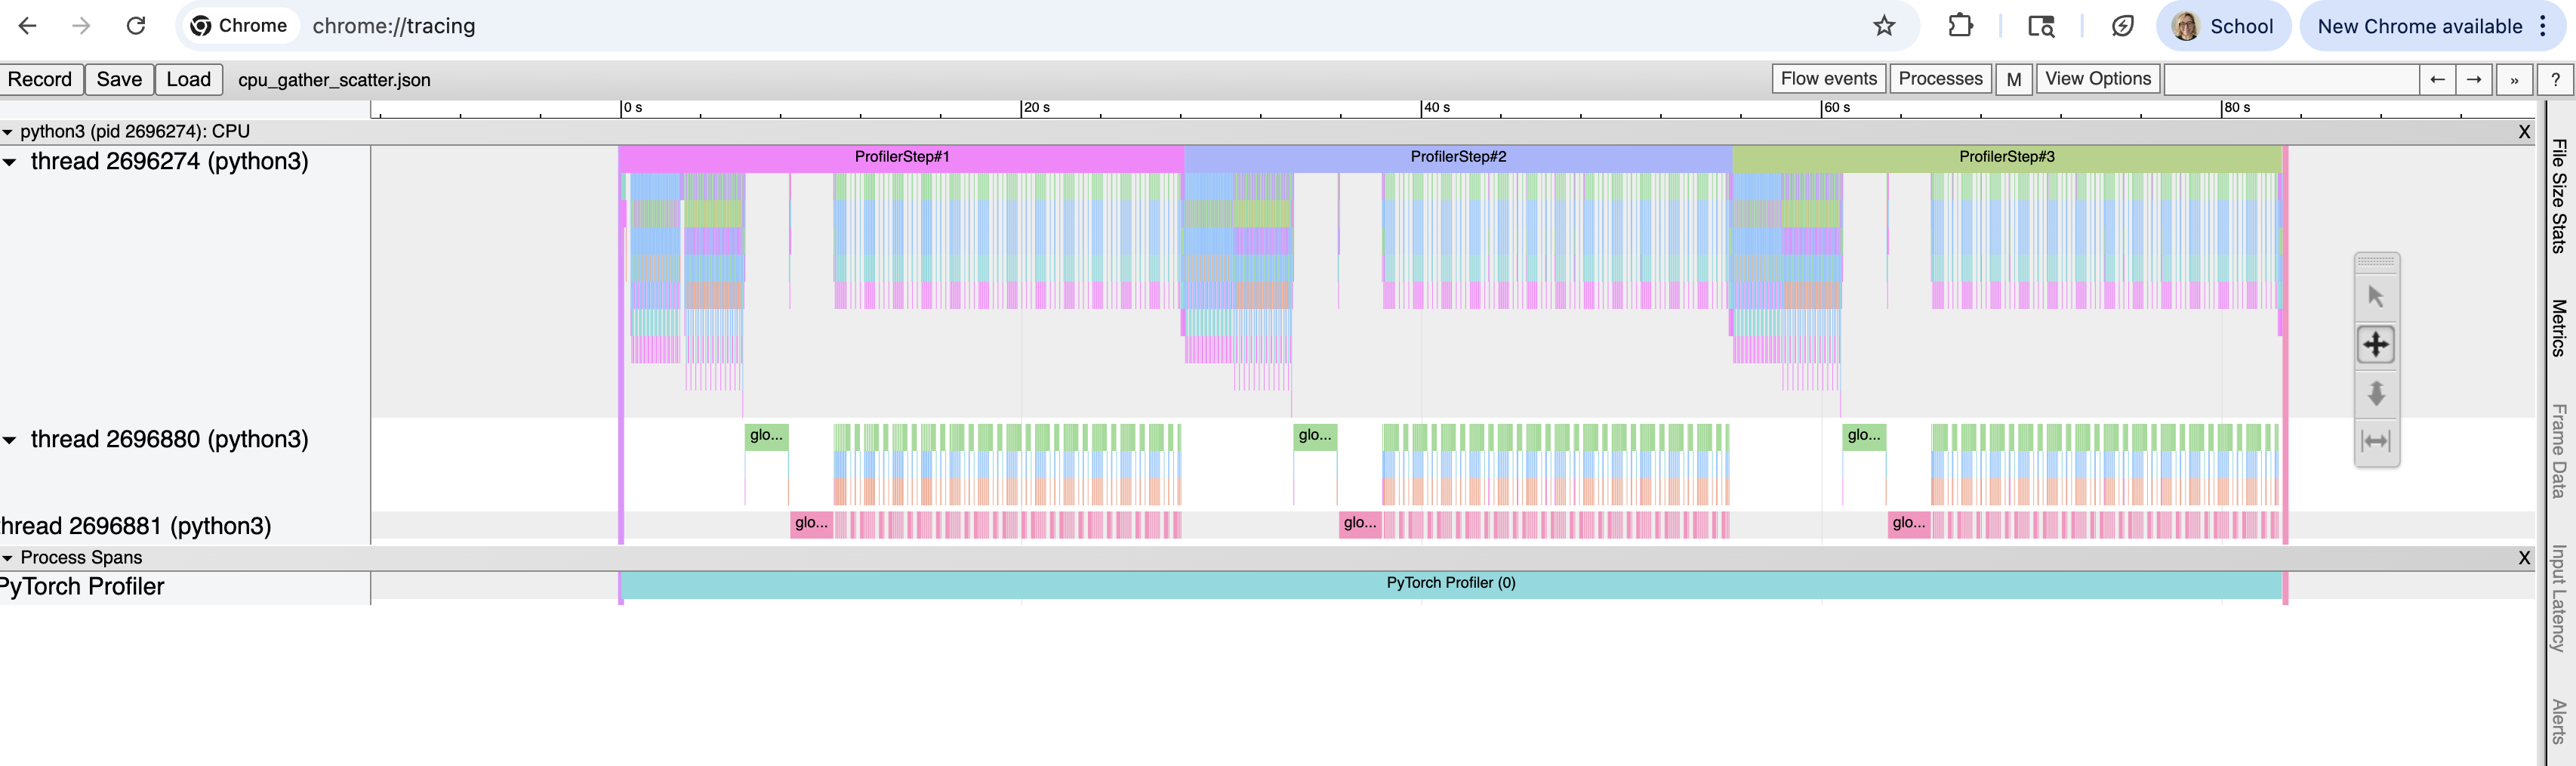
\includegraphics[width=\linewidth]{profiler_images/cpu_gather_scatter.png}
\end{minipage}\hfill
\begin{minipage}[t]{0.48\linewidth}
\centering
\textbf{GPU gather scatter Chrome trace}\\[0.3em]
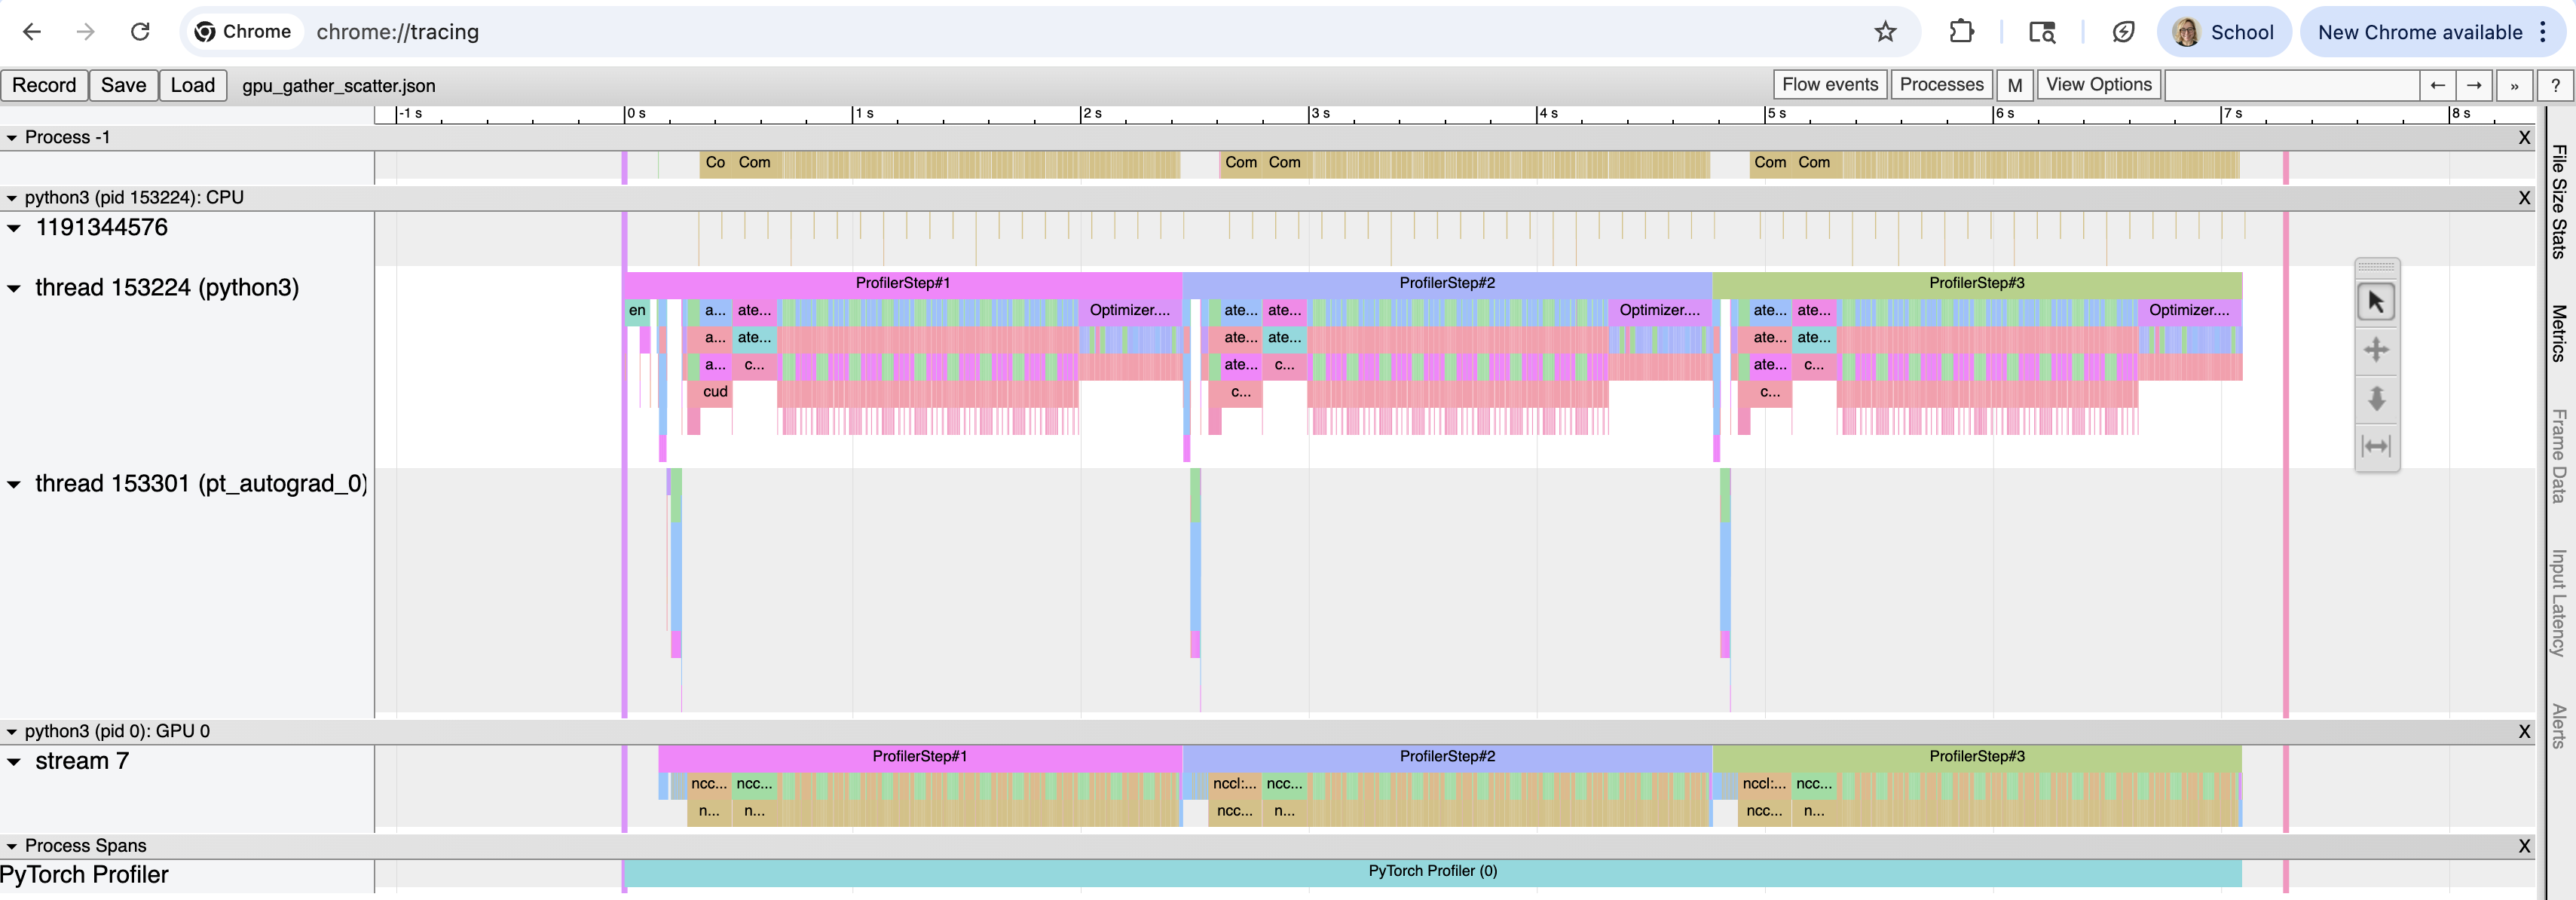
\includegraphics[width=\linewidth]{profiler_images/gpu_gather_scatter.png}
\end{minipage}
\caption{Chrome trace screenshot for gather scatter.}
\end{figure}

\begin{figure}[H]
\centering
\begin{minipage}[t]{0.48\linewidth}
\centering
\textbf{CPU all reduce Chrome trace}\\[0.3em]
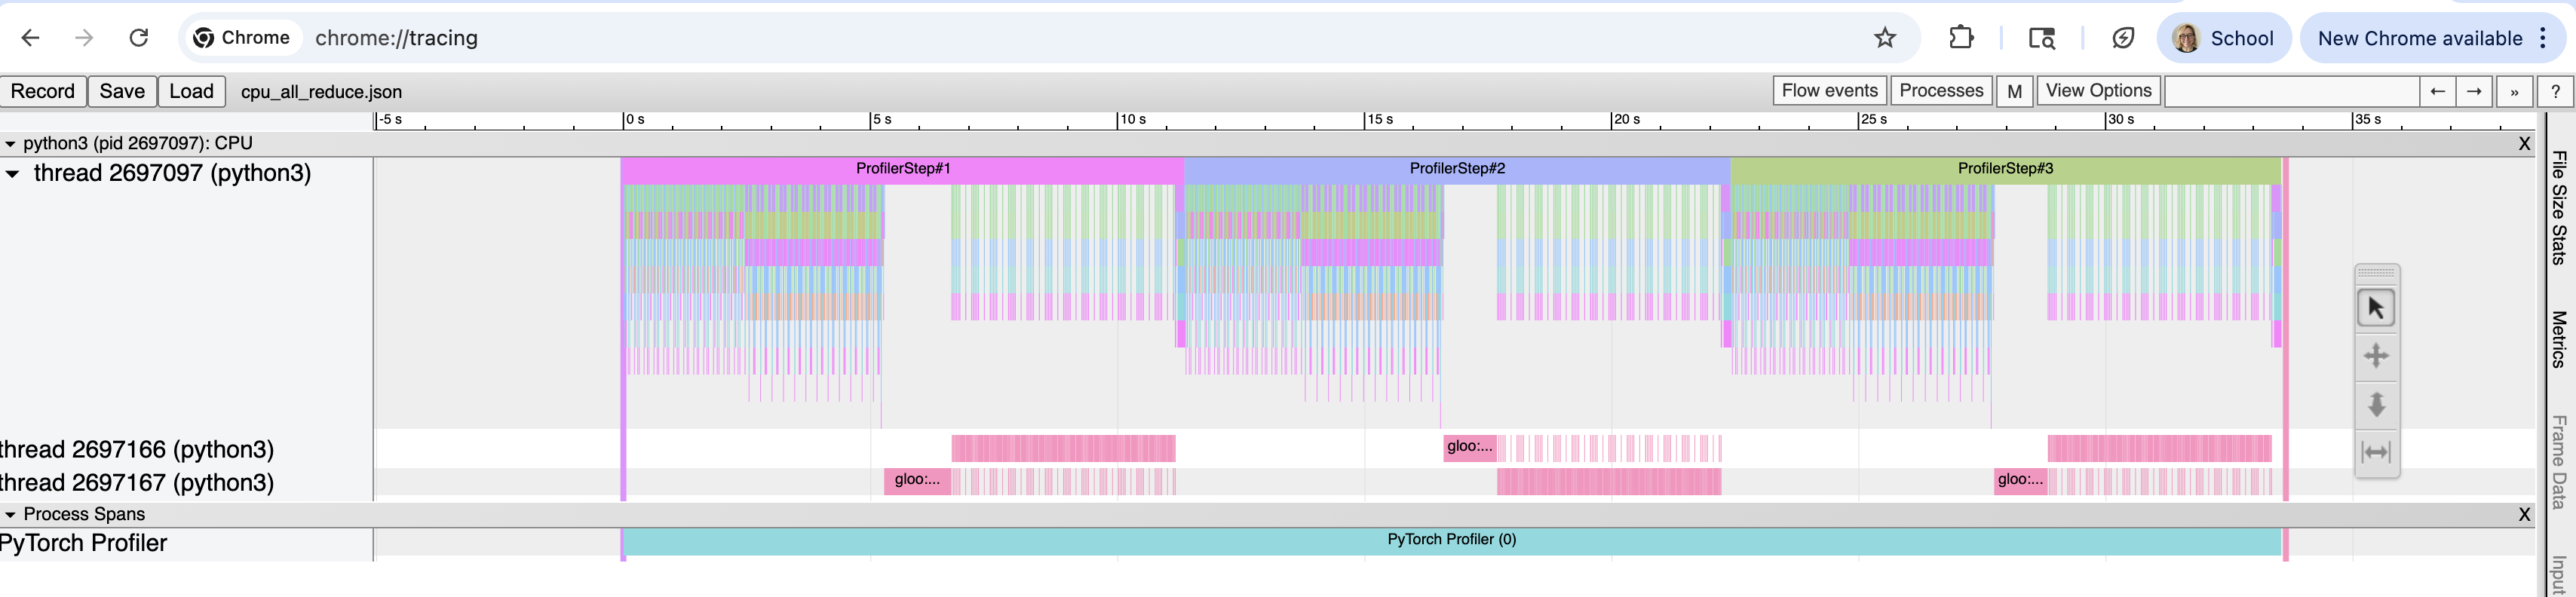
\includegraphics[width=\linewidth]{profiler_images/cpu_all_reduce.png}
\end{minipage}\hfill
\begin{minipage}[t]{0.48\linewidth}
\centering
\textbf{GPU all reduce Chrome trace}\\[0.3em]
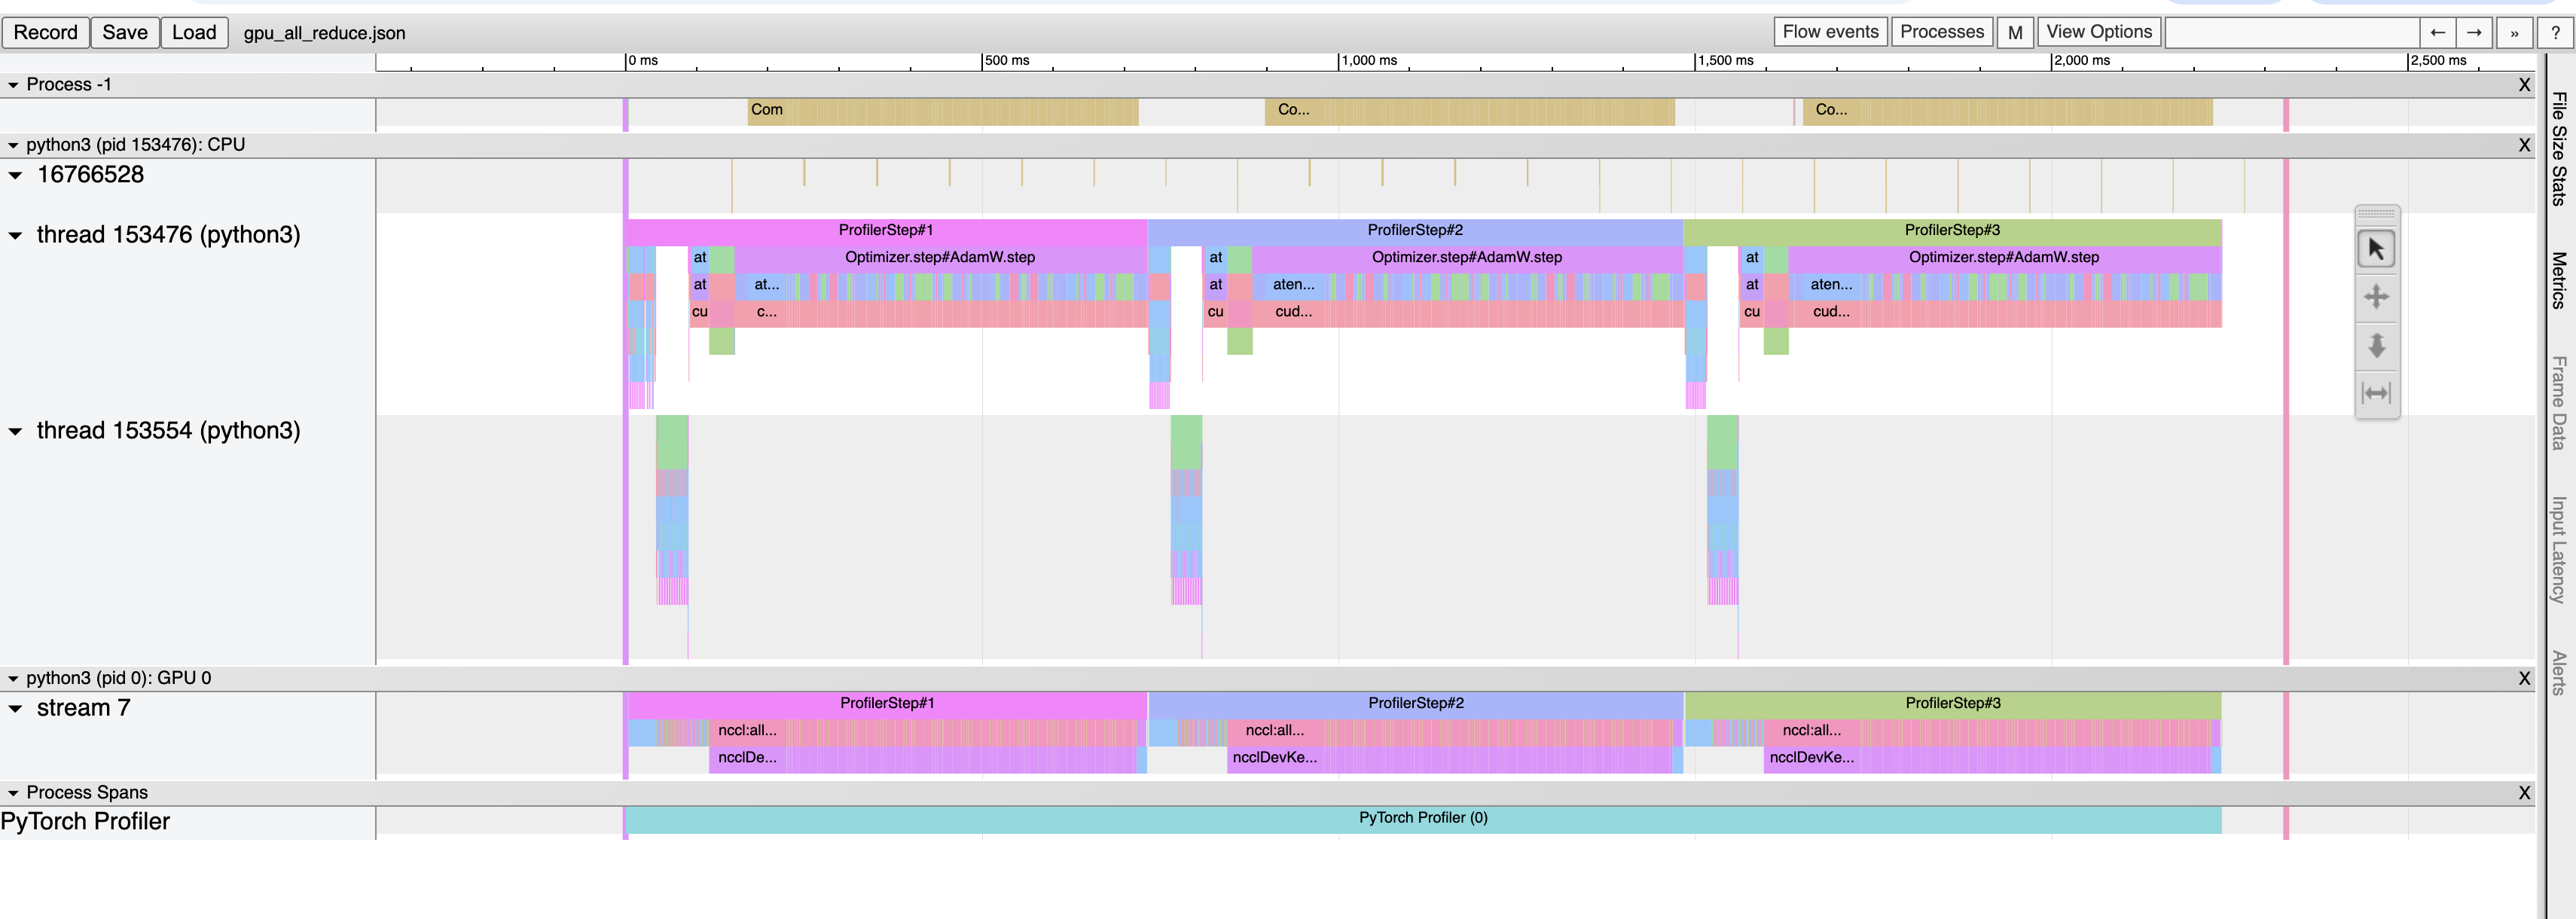
\includegraphics[width=\linewidth]{profiler_images/gpu_all_reduce.png}
\end{minipage}
\caption{Chrome trace screenshot for all reduce.}
\end{figure}

\begin{figure}[H]
\centering
\begin{minipage}[t]{0.48\linewidth}
\centering
\textbf{CPU ddp Chrome trace}\\[0.3em]
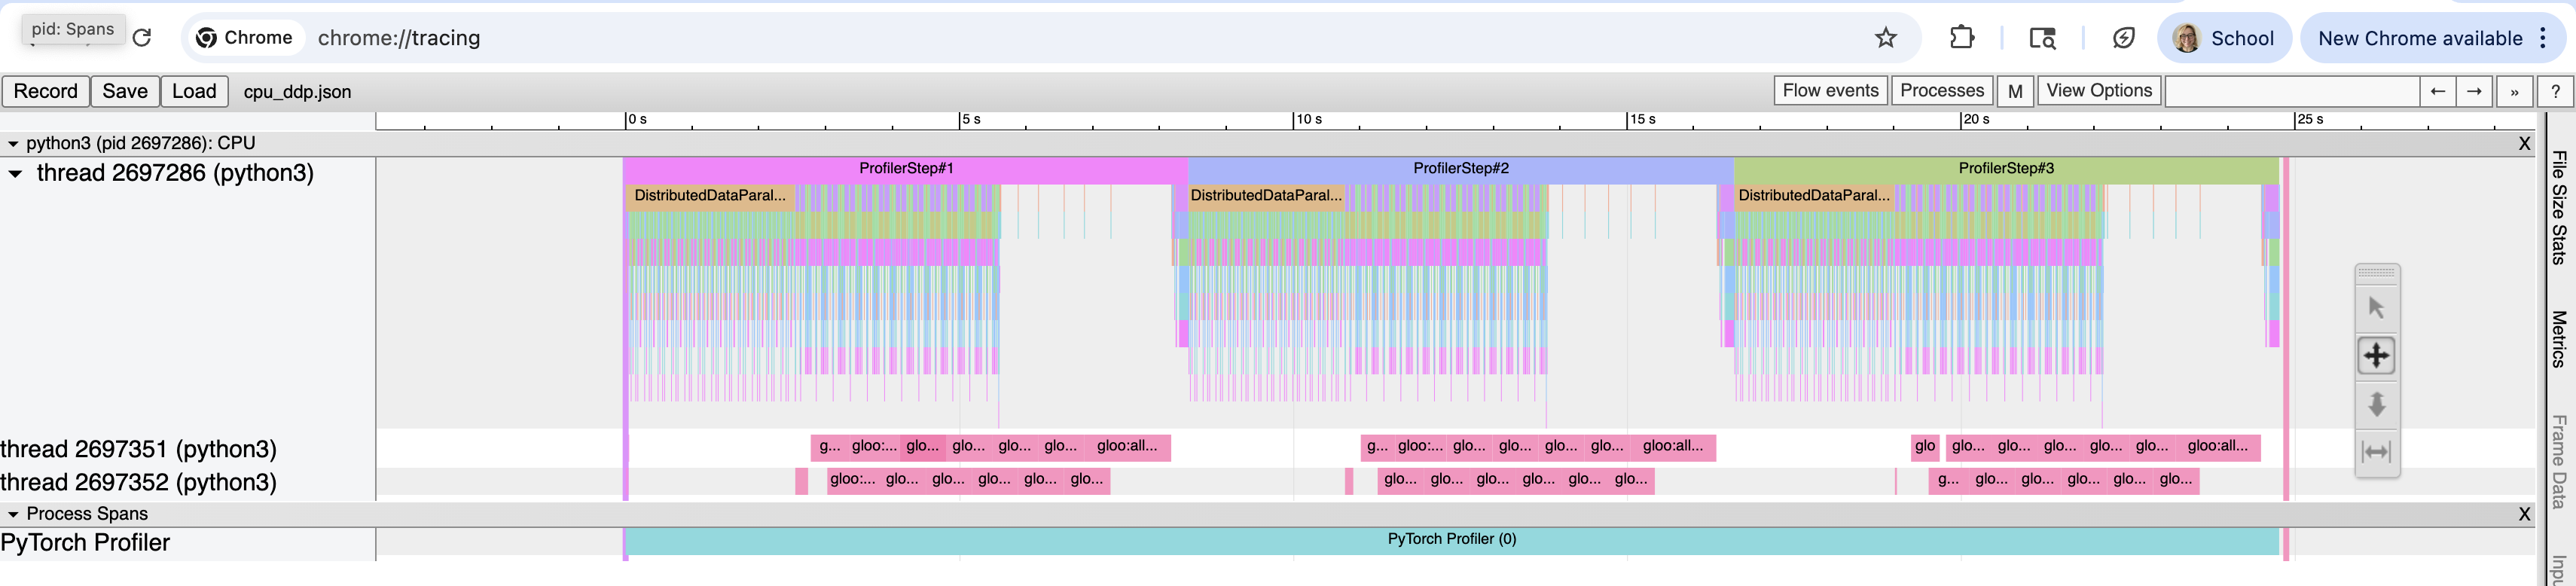
\includegraphics[width=\linewidth]{profiler_images/cpu_ddp.png}
\end{minipage}\hfill
\begin{minipage}[t]{0.48\linewidth}
\centering
\textbf{GPU ddp Chrome trace}\\[0.3em]
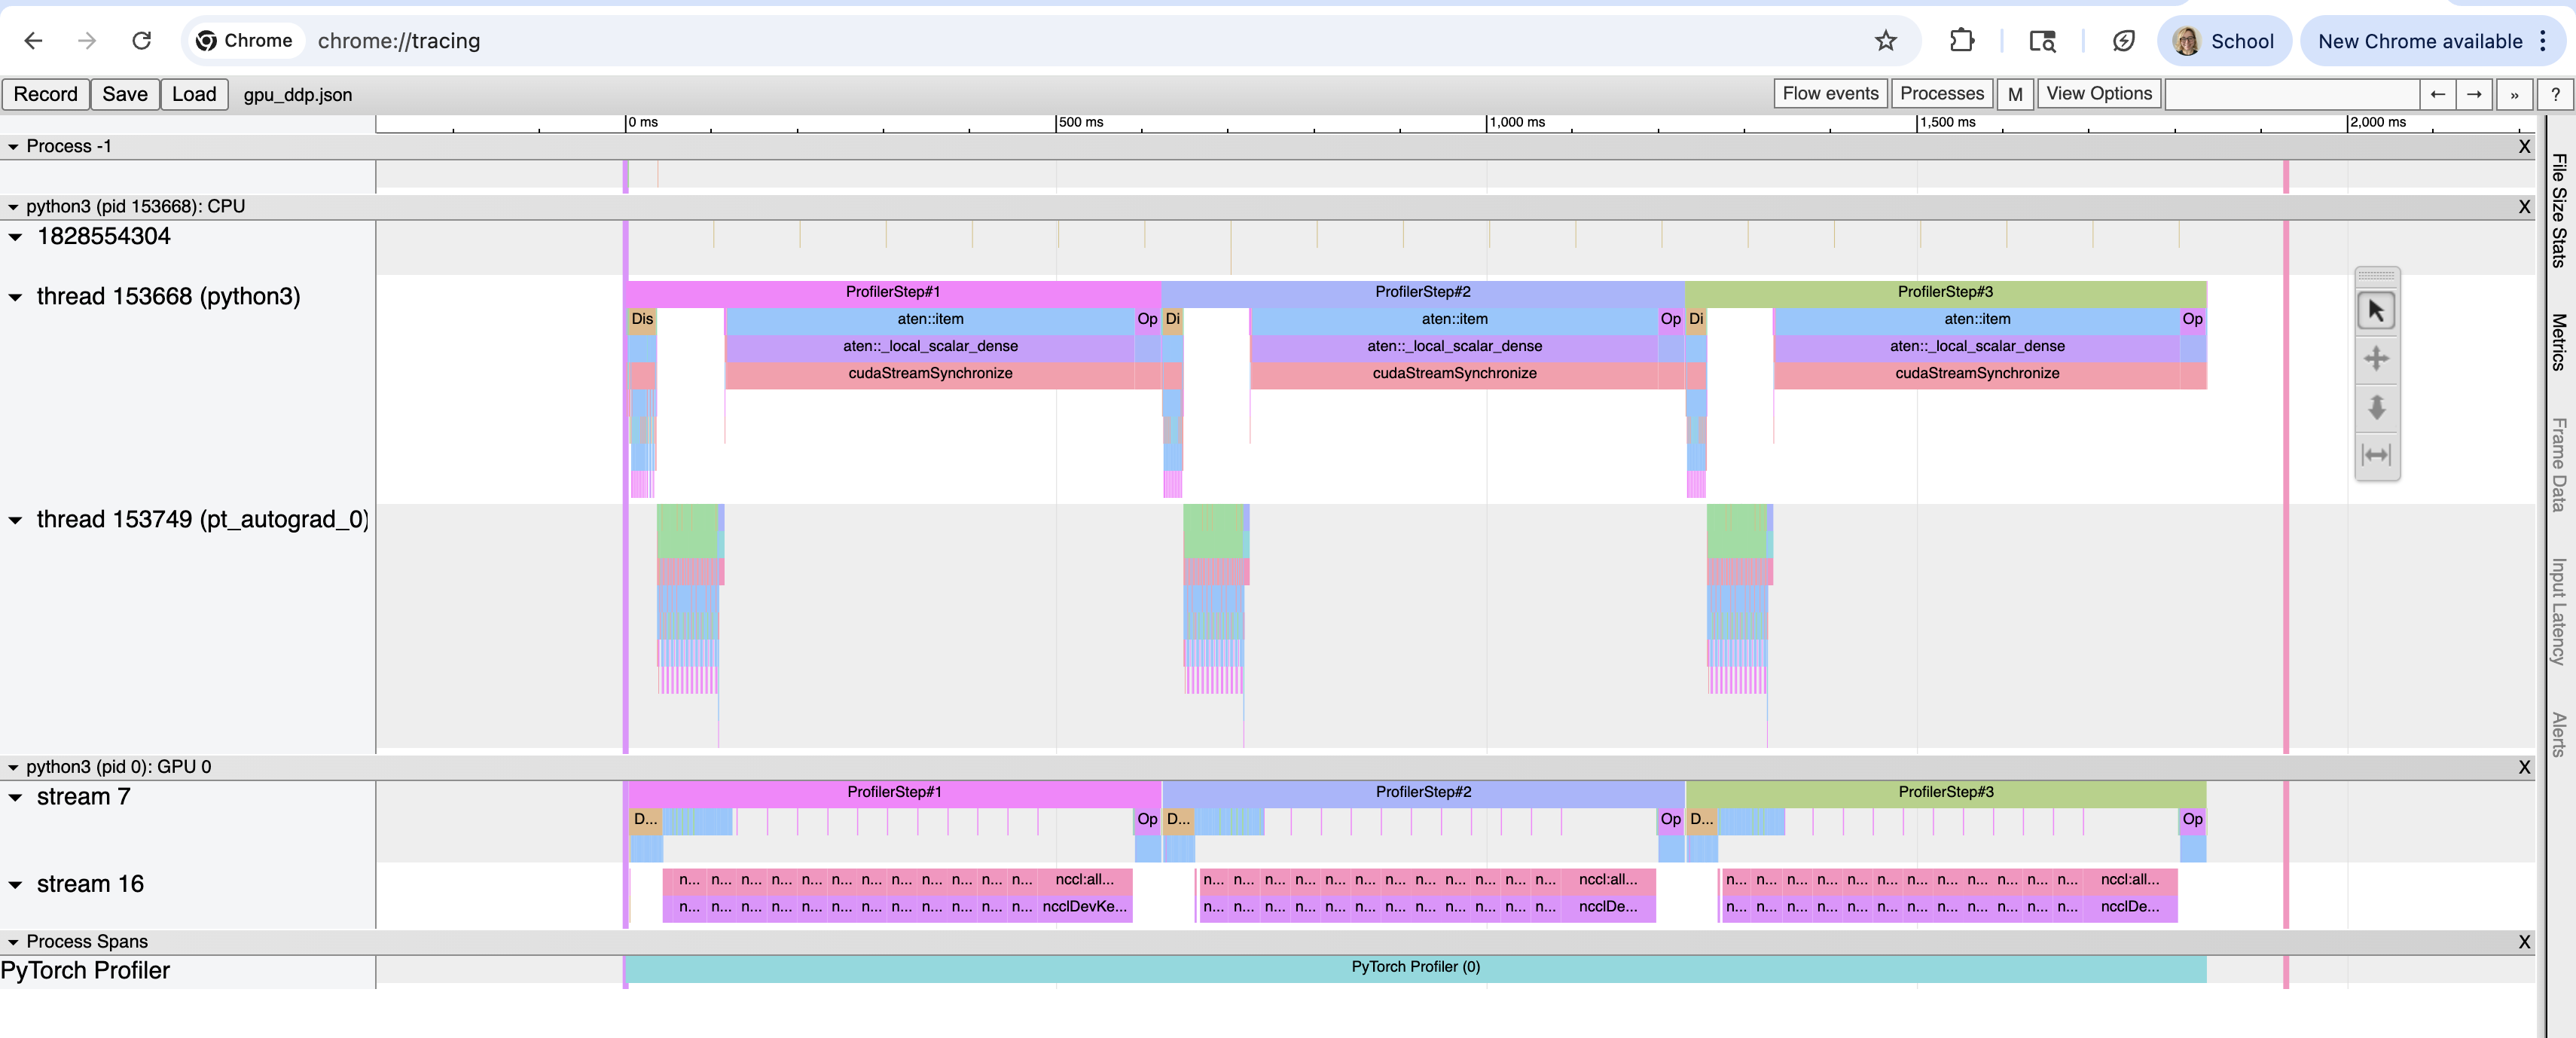
\includegraphics[width=\linewidth]{profiler_images/gpu_ddp.png}
\end{minipage}
\caption{Chrome trace screenshot for ddp.}
\end{figure}

\section{Implementation Details}
The code is organized under \texttt{task1}, \texttt{task2a}, \texttt{task2b}, \texttt{task3}, and \texttt{task4}, matching the deliverable layout requested in the assignment. All distributed runs keep the same total batch size as Task 1 by using per-rank batch size 16 across 4 workers.

Task 1 implements the standard single-node training loop with backward pass, optimizer step, and per-epoch evaluation. Task 2(a) uses a \texttt{DistributedSampler} and manual gradient averaging with \texttt{gather} followed by \texttt{scatter} through rank 0. Task 2(b) replaces that centralized synchronization with \texttt{all\_reduce} and divides by world size on every rank. Task 3 wraps the model in \texttt{DistributedDataParallel}, leaving gradient bucketing and synchronization to PyTorch.

Task 4 reuses the same training code with \texttt{torch.profiler} enabled. The profiler schedule skips the first training step and then records the next three steps (\texttt{wait=1, warmup=0, active=3}), exporting a rank-0 Chrome trace JSON for each communication method.

\section{Discussion}
Across both CPU and GPU, the qualitative ordering is consistent: \texttt{gather}/\texttt{scatter} is slowest, \texttt{all\_reduce} is faster, and \texttt{DistributedDataParallel} is fastest. On CPU, Task 2(b) is 59.16\% faster than Task 2(a), and Task 3 is another 26.23\% faster than Task 2(b). On GPU, Task 2(b) is 68.02\% faster than Task 2(a), and Task 3 is another 20.01\% faster than Task 2(b). The GPU runs are still much faster overall, with GPU/CPU speedups of 11.48x for Task 2(a), 14.66x for Task 2(b), and 13.52x for Task 3.

The Task 2(a) and Task 2(b) loss curves match to within 1.788e-07 on CPU and 1.788e-07 on GPU, which is effectively identical at floating-point precision. That confirms the two manual synchronization implementations are producing the same training trajectory while differing primarily in communication cost.

The lack of difference between Task 2(a) and Task 2(b) in the loss curves is expected. As described in the PyTorch Distributed VLDB'18 paper, distributed data parallel training is designed to be mathematically equivalent to local training when replicas start from the same parameters and synchronize gradients each iteration. In this setup, Tasks 2(a), 2(b), and 3 use the same total batch size and seed, so the main difference among them is communication strategy and runtime cost rather than optimization behavior.

The CPU and GPU runs differ mainly in hardware throughput and backend efficiency rather than in training semantics: GPUs reduce both computation time and collective latency, so the same communication methods preserve ordering but run much faster.

Relative to manual all-reduce, DDP cuts average iteration time by 26.23\% on CPU and 20.01\% on GPU. That end-to-end reduction is the clearest efficiency comparison for Task 4; the corresponding all-reduce gains over gather/scatter are 59.16\% on CPU and 68.02\% on GPU.

The Task 4 communication-share metric is computed on rank 0 as the union of all \texttt{gloo:}/\texttt{nccl:} intervals inside each \texttt{ProfilerStep} window. Under that metric, CPU DDP averages 66.058\% versus 50.527\% for manual all-reduce (+15.531 percentage points), and GPU DDP averages 87.716\% versus 82.569\% (+5.147 points). This does not contradict DDP's better end-to-end time: DDP overlaps reduction with backpropagation and uses optimized gradient buckets, so a larger fraction of a shorter step can still be communication-tagged. This is consistent with the PyTorch Distributed design described in the VLDB'18 paper.

These results also illustrate a practical scalability limit for distributed ML. Better collectives clearly improve throughput, but synchronization still occupies a large share of each profiled step, especially once computation becomes faster. In other words, scaling improves when communication is decentralized and overlapped, but communication overhead does not disappear; it becomes the main factor that limits how close distributed training gets to ideal linear speedup.

\end{document}
